% chapters/06_testing.tex
\chapter{测试与性能分析报告}

\section{概述}

测试是验证系统功能正确性和性能指标的关键环节。本项目采用多层次测试策略，从单元测试到集成测试，从用户态验证到内核态端到端测试，形成了一个完整的测试体系。此外，我们还通过与 Linux 内核的逐字节交叉验证，证明了 Rust 实现与标准实现的行为一致性。

本章首先介绍测试架构的总体设计，然后依次展示功能正确性测试、性能基准测试、启动开销分析和 Linux 交叉验证的结果。所有原始数据、CSV 和串口日志均已版本化归档至 \texttt{docs/evidence/}，可供复核。

\section{测试架构概述}

测试基础设施弥合了 Rust 实现与现有行业标准（如 Linux 中的 dm-crypt 和 dm-verity）之间的差距。整个测试体系分为四个层级：

\begin{table}[H]
    \centering
    \caption{测试层级划分}
    \label{tab:test_layers}
    \begin{tabular}{p{0.22\textwidth}p{0.35\textwidth}p{0.35\textwidth}}
        \toprule
        \textbf{测试层级} & \textbf{范围} & \textbf{关键组件} \\
        \midrule
        单元测试 & 单个结构体的逻辑验证 & \texttt{FileBlockDevice}、\texttt{DmCryptDevice}、\texttt{HashTree} \\
        集成测试 & Rust 工作空间内的端到端流程 & \texttt{dmctl demo} 命令 \\
        交叉验证 & 与 Linux 内核标准的兼容性 & 验证脚本、\texttt{cryptsetup} \\
        内核端到端 & 在星绽操作系统内部进行的功能测试 & \texttt{VirtioBlkAdapter}、\texttt{pivot\_root} 流程 \\
        \bottomrule
    \end{tabular}
\end{table}

\begin{figure}[H]
    \centering
    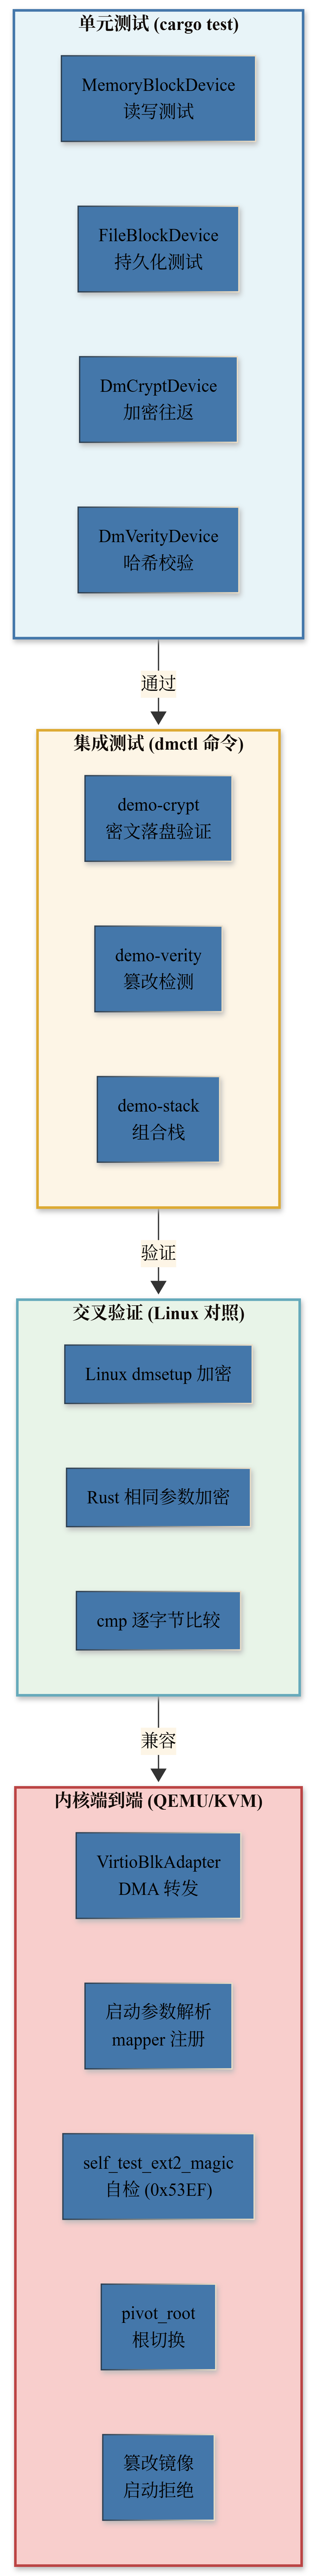
\includegraphics[width=0.9\textwidth]{figures/test_execution_flow.png}
    \caption{测试执行与数据流图}
    \label{fig:test_execution}
\end{figure}

\section{功能正确性测试}

功能正确性是比赛评审的核心指标（占 50\%）。我们针对 dm-verity 和 dm-crypt 分别设计了严格的功能测试。

\subsection{dm-verity 完整性校验测试}

\subsubsection{正常启动验证}

在正常场景下，系统使用正确的根哈希启动，能够成功挂载受 dm-verity 保护的根文件系统。验证步骤如下：

\begin{enumerate}
    \item 使用 \texttt{scripts/build\_verity\_rootfs.sh} 构建包含默克尔树的 ext2 镜像（数据块数 65536，哈希树从块号 65536 开始）。
    \item 通过 QEMU/KVM 启动星绽内核，传递 verity 相关启动参数（\texttt{rootfs\_verity.scheme=dm-verity}，\texttt{rootfs\_verity.hash=<root\_hash>}，\texttt{rootfs\_verity.data\_blocks=65536}，\texttt{rootfs\_verity.hash\_start=65536}，\texttt{rootfs\_verity.cache\_blocks=256}）。
    \item 系统在初始化阶段创建 \texttt{DmVerityDevice} 映射器，执行 \texttt{self\_test\_first\_block} 自检（验证第一个数据块）。
    \item 自检通过后，initramfs 使用 \texttt{dm-root} 模式将映射器挂载到 \texttt{/newroot}，执行 \texttt{pivot\_root} 切换根目录。
    \item 串口日志输出 \texttt{[dm-test] PASS first data block verified through dm-verity} 和 \texttt{PASS system root switched to protected mapper}，并输出 verity 统计信息（\texttt{verified}、\texttt{hash\_hits}、\texttt{hash\_misses} 等）。
\end{enumerate}

版本化证据位于 \texttt{docs/evidence/asterinas-verity-rootfs-kvm.log}，串口确认 \texttt{status=verified}。

\subsubsection{篡改检测测试}

为了验证 dm-verity 的防篡改能力，我们构造了恶意修改的块设备数据：

\begin{enumerate}
    \item 在底层镜像的数据块 0 的偏移 0 处将字节 XOR 0xff（仅修改一个字节）。
    \item 使用相同的根哈希启动星绽内核。
    \item 系统在自检阶段（\texttt{self\_test\_first\_block}）检测到完整性违规，映射器注册失败。
    \item 内核记录 \texttt{VERITY\_BOOT\_STATUS=integrity-rejected}，串口输出 \texttt{[dm-test] FAIL dm-verity rejected first data block: IntegrityViolation}。
    \item 无任何 \texttt{root switch PASS} 标记，系统 panic 或停止。
\end{enumerate}

证据位于 \texttt{docs/evidence/asterinas-verity-rootfs-tampered-kvm.log}，确认 \texttt{status=integrity-rejected} 且无成功根切换。

\subsection{dm-crypt 透明加密测试}

\subsubsection{加密往返测试}

加密往返测试验证了加密的基本安全属性：

\begin{enumerate}
    \item 创建 \texttt{MemoryBlockDevice} 作为底层设备（4 块，每块 64 字节）。
    \item 用密钥 \texttt{b"demo-key"} 将其包装在 \texttt{DmCryptDevice} 中。
    \item 向块 1 写入明文 \texttt{b"hello from dm-crypt minimal demo block, padded for testing......"}。
    \item 从底层设备读取块 1 的数据，确认呈现为密文（与明文不同，且不包含 \texttt{b"hello"} 子串）。
    \item 通过 \texttt{DmCryptDevice} 读取块 1，确认恢复为原始明文。
\end{enumerate}

该测试在 \texttt{crates/dm/tests/crypt\_test.rs} 中实现，通过 \texttt{cargo test} 自动执行。

\subsubsection{密钥分离测试}

密钥分离测试验证了密钥的正确性要求：

\begin{enumerate}
    \item 使用密钥 \texttt{b"right-key"} 加密数据并写入块 0。
    \item 使用不同的密钥 \texttt{b"wrong-key"} 初始化 \texttt{DmCryptDevice} 并读取同一块。
    \item 预期结果：读取到的数据与原始明文不匹配。
\end{enumerate}

该测试确保错误的密钥无法恢复明文，体现了密码学安全的正确性。

\subsection{Linux 兼容性验证}

为确保与 Linux \texttt{aes-xts-plain64} 的逐字节兼容，我们运行了交叉验证脚本 \texttt{scripts/verify\_linux\_xts\_compat.sh}：

\begin{enumerate}
    \item 在 Linux 下使用 \texttt{dmsetup} 创建 crypt 映射（\texttt{aes-xts-plain64}，64 字节密钥），写入特定位模式（全 0x5a）。
    \item 在 Rust 中使用 \texttt{dmctl crypt-table-fill} 使用相同密钥和参数，写入相同模式。
    \item 使用 \texttt{cmp} 比较两个密文扇区，确保完全相同。
\end{enumerate}

版本化向量 SHA-256 保存在 \texttt{docs/evidence/linux-xts-plain64.sha256} 中，固定为 \texttt{4334c17f4b0380b3c1f902509cce0c0f98d9fa77aa93f6407ec940215d77921d}。

\subsection{内核端到端功能验证}

在 Asterinas 内核中，我们还验证了以下端到端场景：

\begin{itemize}
    \item \textbf{动态控制面}：通过 \texttt{/dev/mapper/control} 的 \texttt{dm\_ioctl} 接口，使用 \texttt{cryptsetup 2.7.5} 完成 \texttt{open}（创建 mapper）、\texttt{read}（验证可读性）和 \texttt{close}（删除 mapper）的完整流程。
    \item \textbf{受保护根文件系统}：dm-crypt 加密根和 dm-verity 校验根分别通过 \texttt{pivot\_root} 切换成功。
\end{itemize}

证据见 \texttt{docs/evidence/asterinas-cryptsetup-aesni-kvm.log} 和 \texttt{docs/evidence/asterinas-crypt-rootfs-aesni-kvm.log}。

\section{性能基准测试}

性能是比赛评审的另一个重要维度（Demo 质量占 20\%）。我们按照正式合同进行了全面的 I/O 性能评估。

\subsection{正式测试合同}

所有内核性能数据均遵循以下不可省略的合同：

\begin{table}[H]
    \centering
    \caption{正式性能测试合同}
    \label{tab:test_env}
    \begin{tabular}{p{0.30\textwidth}p{0.60\textwidth}}
        \toprule
        \textbf{配置项} & \textbf{固定值} \\
        \midrule
        内核构建 & \texttt{release-lto}（含链接时优化） \\
        虚拟化 & KVM，CPU=host，1 vCPU，8 GiB 内存 \\
        块设备 & virtio-blk，264 MiB 容器，测试前 256 MiB \\
        fio 负载 & 顺序读（read），4 KiB，sync，direct=1，QD1 \\
        时长 & 2 秒 ramp + 10 秒 runtime \\
        重复轮次 & raw/target 交替顺序，各五轮 \\
        阶段统计 & \texttt{dm.perf\_stats=1} 开启细粒度归因 \\
        \bottomrule
    \end{tabular}
\end{table}

执行命令：
\begin{lstlisting}[basicstyle=\ttfamily\small]
sudo bash scripts/run_formal_dm_benchmark.sh --build-images
\end{lstlisting}

该命令构建加密和 verity 镜像，在 KVM 中交替运行 raw/dm-crypt/dm-verity 各五轮，生成统一三行结果表和阶段归因 CSV。

\subsection{I/O 性能测试结果}

五轮中位数结果如下：

\begin{table}[H]
    \centering
    \caption{正式性能基准结果}
    \label{tab:formal_results}
    \begin{tabular}{p{0.20\textwidth}p{0.20\textwidth}p{0.20\textwidth}p{0.20\textwidth}}
        \toprule
        \textbf{设备} & \textbf{中位吞吐（MiB/s）} & \textbf{中位 p95（us）} & \textbf{相对配对 raw} \\
        \midrule
        raw（两组共十轮） & 4.249 & 1277.952 & 100.0\% \\
        dm-crypt & 4.059 & 1318.912 & 95.6\% \\
        dm-verity & 3.815 & 1433.600 & 87.3\% \\
        \bottomrule
    \end{tabular}
\end{table}

阶段归因显示 dm-crypt 的下层等待占 97.84\%，AES-XTS 占 1.82\%；dm-verity 的下层等待占 93.01\%，数据 SHA-256 占 5.74\%。未归因部分分别为 0.14\%--0.15\%（crypt）和 0.23\%--0.33\%（verity）。因此当前瓶颈明确为下层 I/O 等待，而非密码计算或缓存策略。原始 CSV、metadata 和阶段数据位于 \texttt{docs/evidence/formal-256m/}。

\subsection{启动开销分析}

启动时间测量评估了引入 dm-verity 后对内核启动时间的影响。使用交替顺序五轮冷启动测试，从 QEMU 启动到串口出现 \texttt{PASS system root switched to protected mapper} 为止。

\begin{table}[H]
    \centering
    \caption{根文件系统启动时间}
    \label{tab:boot_time}
    \begin{tabular}{p{0.30\textwidth}p{0.25\textwidth}p{0.35\textwidth}}
        \toprule
        \textbf{场景} & \textbf{五轮中位数（秒）} & \textbf{增量} \\
        \midrule
        plain root & 16.058 & — \\
        dm-verity root & 16.902 & +5.256\% \\
        \bottomrule
    \end{tabular}
\end{table}

逐轮 CSV 和串口日志位于 \texttt{docs/evidence/asterinas-boot-time-kvm.csv} 及对应日志目录。

\subsection{Linux guest 与 Asterinas 同条件对照}

为了进行公平的跨系统比较，我们使用同一宿主机、同一 raw 数据盘、相同的 QEMU/KVM 配置，分别启动 Linux 和 Asterinas 运行相同 fio 合同。比较器强制核对 vCPU、内存、加速器、CPU 模型、设备模型、测试区域 SHA-256、密码参数和 fio 参数，任一项不同则拒绝出表。

结果如下：

\begin{table}[H]
    \centering
    \caption{Linux guest vs Asterinas dm-crypt 同条件五轮对照}
    \label{tab:linux_asterinas}
    \begin{tabular}{p{0.20\textwidth}p{0.20\textwidth}p{0.20\textwidth}p{0.15\textwidth}p{0.15\textwidth}}
        \toprule
        \textbf{系统} & \textbf{raw MiB/s} & \textbf{dm-crypt MiB/s} & \textbf{保留率} & \textbf{p95 us} \\
        \midrule
        Linux guest & 5.150 & 4.746 & 92.158\% & 1384.448 \\
        Asterinas & 4.245 & 4.059 & 95.621\% & 1318.912 \\
        \bottomrule
    \end{tabular}
\end{table}

Asterinas raw 和 dm-crypt 的绝对吞吐分别为 Linux guest 的 \textbf{82.4\%} 和 \textbf{85.5\%}。保留率以各系统自身 raw 为基线，Asterinas 的较高保留率不代表绝对吞吐超过 Linux。详细比对见 \texttt{docs/evidence/linux-vs-asterinas-dm-crypt.md}。

\section{创新技术验证}

针对比赛要求的“技术探索”指标（占 10\%），我们对提出的可信存储性能优化技术进行了专项验证：

\begin{table}[H]
    \centering
    \caption{哈希块缓存效果验证}
    \label{tab:cache_validation}
    \begin{tabular}{p{0.20\textwidth}p{0.25\textwidth}p{0.25\textwidth}p{0.20\textwidth}}
        \toprule
        \textbf{场景} & \textbf{中位吞吐（MiB/s）} & \textbf{中位 p95（us）} & \textbf{hash hits/misses} \\
        \midrule
        无缓存（cache=0） & 0.320 & 15007.744 & 0 / 2420 \\
        有缓存（cache=256） & 0.398 & 13697.024 & 2785 / 5 \\
        \bottomrule
    \end{tabular}
\end{table}

缓存提升中位吞吐 \textbf{24.4\%}，降低 p95 \textbf{8.7\%}。两组均为 \texttt{data\_rereads=0}，证明收益来源于减少 Merkle hash block 重读，而非跳过数据认证。原始数据位于 \texttt{docs/evidence/asterinas-verity-fio-cache0-kvm.csv} 和 \texttt{asterinas-verity-fio-cache256-kvm.csv}。

\section{证据可复核性}

所有性能数据均遵循以下可复核要求：

\begin{itemize}
    \item 每个工况至少五轮，交替执行 raw 和目标设备。
    \item 报告中位数、p50、p95、p99，不选择最好的一轮。
    \item 每轮 fio 前后读取 \texttt{/proc/dm-performance-stats}，使用差值计算阶段耗时。
    \item 所有原始 CSV、metadata 和串口日志均已归档至 \texttt{docs/evidence/}，按场景分类。
    \item metadata 包含 git commit、dirty 状态、构建 profile、KVM/CPU 配置、镜像 SHA-256 和 fio 参数，确保可复现。
\end{itemize}

\section{小结}

本章展示了项目的测试与验证体系。在功能正确性方面，dm-verity 的篡改检测和 dm-crypt 的透明加密均通过了端到端测试；性能部分通过正式合同给出了可复现的基准数据，包括 raw、dm-crypt、dm-verity 三行表及 Linux guest 同条件对照；启动开销和哈希缓存优化也提供了量化证据。在交叉验证方面，与 Linux 内核的逐字节兼容性验证证明了密码格式兼容。所有原始 CSV、metadata 和串口日志均已归档至 \texttt{docs/evidence/} 供复核。